% ----------------------------------------------------------
% revisão bibliográfica
% ----------------------------------------------------------
\chapter[Revisão Bibliográfica]{Revisão Bibliográfica}

Este capítulo apresenta um levantamento bibliográfico sobre segurança da informação e vulnerabilidades. Tem como objetivo definir conceitos e apresentar exemplos da utilização dos termos e seus exemplos no mundo real. Será listada as definições e as ténicas utilizadas para efetuar o trabalho e como serão considerados os dados para sua utilização posterior. Será considerado ainda as ferramentas a ser utilizadas para a busca da pesquisa.

% --------------------------%
% --- Conceitos Básicos --- %
\section{Segurança da Informação}

Segurança da Informação é o conjunto de orientações, normas, procedimentos, políticas e demais ações que têm por objetivo proteger o recurso informação, possibilitando que o negócio da organização seja realizado e a sua missão seja alcançada \cite{Fontes2017}. Assim, a segurança é o pilar principal de pesquisa desse trabalho.  Quando se envolve segurança de sistemas, de redes, de serviços etc; se resume tudo em segurança da informação.  

Proteger a informação é responsabilidade de cada usuário na organização em que coopera e cabe à organização orientar seus colaboradores em relação à proteção da informação. De acordo com \citeonline{Spanceski2004}, uma das formas de proteger a informação é conhecer os pilares da área da segurança da informação. Esses, são considerados as divisões dessa ciência que juntos formam toda a segurança da informação. São:

\begin{itemize}
\item Integridade: pilar que assegura que sistemas e informações serão modificados apenas nas condições previstas, assim impede que sejam manipuladas afetando os usuários. A integridade é a garantia da exatidão e completeza da informação e dos métodos de processamento \cite{ABNT2005};
\item Disponibilidade: garante que os dados, sistemas e serviços estejam disponíveis para aqueles que tem o direito de utilizá-los. A disponibilidade é a garantia de que os usuários autorizados obtenham acesso à informação e aos ativos correspondentes sempre que necessário \cite{ABNT2005}.
\item Confidencialidade: esse pilar assegura que as informações não serão acessadas por agentes não autorizados. A confidencialidade é a garantia de que a informação é acessível somente por pessoas autorizadas a terem acesso \cite{ABNT2005}.
\end{itemize}

A integridade de uma mensagem A é o conceito de que não há nenhuma alteração em seu conteúdo mantendo sua estrutura original. Garantir sua integridade significa não permitir que a informação seja modificada, alterada ou mesmo destruída, que seja legítima e permancessa consistente \cite{Dantas2011}.

Ocorre a não integridade de uma informação quando seu conteúdo é corrompido, falsificado, roubado ou destruído \cite{Dantas2011}. Quando uma informação está íntegra, então seus dados são seguros e há a garantia que são originais.

A disponibilidade reporta a garantia de que uma informação está acessível. Deste modo, não se restringe apenas a algum sistema online estar apto a se conectar, mas uma informação que esteja ao alcance dos usuários destinatários.

Quando não há disponibilidade significa que a informação não está disponível para ser utilizada, ou seja, está fora do alcance dos usuários destinatários \cite{Dantas2011}. 

Para ter disponibilidade deve ser assegurando a garantia da leitura e acesso da informação no momento em que se necessita da mesma.

A confidencialidade é a certeza de que uma informação é acessível apenas para o remetente e para o destinatário, sendo que qualquer outro terceiro não consiga ter a informação encaminhada. A garantia da confidencialidade é deixar de que outro terceiro não tenha acesso à informação original e que não possa divulga-la. 

É natural que com a evolução e o desenvolvimento a segurança da informação tenha se focado muito na área de comunicação de dados e informação. Esse fato, abre porta para outras pontas de atenção, como:

\begin{itemize}
\item Autenticidade: garante que a mensagem é do próprio remetente. É a garantia de que a informação é oriunda da fonte que lhe é atribuída e elaborada por quem tem autoridade para tal. Diz respeito à idoneidade da fonte, ou seja, digna de confiança \cite{Dantas2011};
\item Confiabilidade: garante que a fonte emitente da mensagem é confiável e autêntica. É a garantia de que a informação é confiável, oriunda de uma fonte autêntica e que expressa uma mensagem verdadeira. Diz respeito ao conteúdo \cite{Dantas2011}.
\item Não repúdio: garante que a informação sempre chegará ao destino final e será sempre interpretada. É a garantida de que a informação chegará ao destino certo e não será repudiada. \cite{Dantas2011}.
\item Responsabilidade: é o agregado de responsabilidade de todos os envolvidos na criação, armazenamento e transporte da informação. É a coparticipação de responsabilidades por todos os que produzem, manuseiam, transportam e descartam a informação, seus sistemas e redes de trabalho. \cite{Dantas2011}.
\end{itemize}

Com esse conjuto de propriedades presente na comunicação em rede \cite{ABNT2005}, o remetente tem a garantia de quem recebe suas informações é realmente o destinatário que se diz ser. Garante ainda que a informação recebida está exatamente igual à enviada pelo remetente. Assegura também que nem o emissor nem o remetente neguem que houve comunicação.

\section{Vulnerabilidades de Segurança}
A quebra da segurança da informação indica que um sistema ou serviço foi violado, ou seja, algo em sua essência possibilitou que algum atacante conseguice penetrar em suas camadas a ponto de encontrar uma forma de roubar uma informação, por exemplo. Isso é considerado uma vulnerabilidade do sistema. 

No contexto de segurança da informação, vulnerabilidade pode ser uma falha em um sistema ou serviço que permita realização e concretização de um ataque \cite{Aparecido2014}. Para que um atacante consiga explorar essa vulnerabilidade, ele precisa de um meio ou ferramentas que possibilite seu ataque, assim ele conecta com a fraqueza do sistema ou serviço, essas ferramentas ou mesmo tecnicas são chamadas de exploits \cite{Whitman2011}.

A figura \ref{fig:xiao} representa o ciclo de vida de uma vulnerabilidade. De modo geral, uma vulnerabilidade tem o seu descobrimento e, a partir disso, há os passos para soluciona-lo. Representando um sistema que esteja já em base de produção, a vulnerabilidade se destaca como um bug, mas não um simples bug, mas sim um que tenha postencial de afetar o sistema. No modo de produção do sistema, a equipe então desenvolverá uma versão que corrija aquele bug e liberará essa correção, seja como um instalador de sistema, para aplicativos desktop ou mesmo para mobile, ou então irá subir no servido, caso seja um site ou serviço de API. 

\begin{figure}[H]
\centering
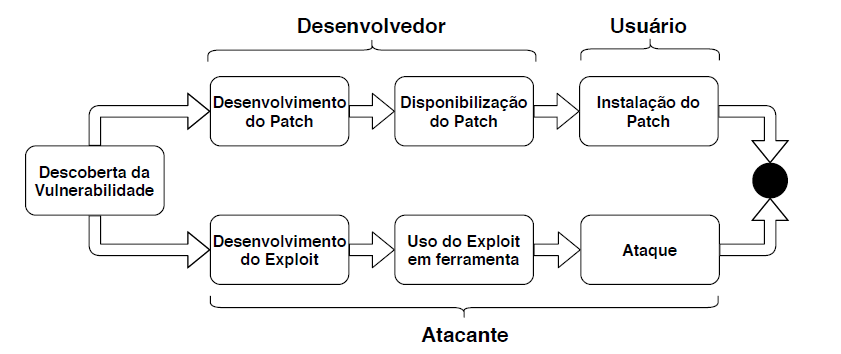
\includegraphics[width=1\textwidth]{imagens/figura_xiao.PNG}
\caption{Ciclo de vida de uma vulnerabilidade \cite{xiao2018patching}}
\label{fig:xiao}
\end{figure}

O ciclo de vida de um software é vinculado com essa parte de desecoberta de vulnerabilidades, muita das vezes é até previsto no projeto. Quando se encontra algum bug ou backdoor que leve a algum ponto crítico de atenção, a equipe de desenvolvimento do sistema, serviço ou software, tem a responsabilidade de disponibilizar uma nova versão tal que a correção seja disponibilizada.

Existe ainda as ameaças que o software pode enfrentar, dessas são descobratas as vulnerabilidades. A saber \cite{Pfleeger2015}:

\begin{itemize}
\item Falhas no software ou no Hardware. Desde parâmetros externos, como fator ambiental, a fator interno como falta de memória.
\item Erros de usabilidade ou falha de administração.
\item Erros no projeto e de implementação.
\end{itemize}

Em sumo, não é possível a construção de uma lista que contenha todas as possíveis ameaças existentes. As formas de se encontrar vulnerabilidades em sistemas é diferente em cada tentativa e identificação de vulnerabilidade \cite{Pfleeger2015}. Como exemplo, o livro \citeonline{Pfleeger2015} apresenta a figura \ref{fig:vulnerabilidadeAgua} que faz uma analogia de uma vulnerabilidade do sistema.

\begin{figure}[H]
\centering
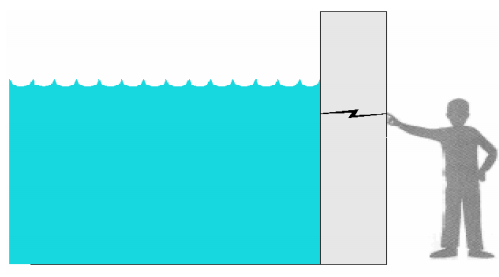
\includegraphics[width=1\textwidth]{imagens/vulnerabilidadeAgua.png}
\caption{Ameaça e Vulnerabilidade \cite{Pfleeger2015}}
\label{fig:vulnerabilidadeAgua}
\end{figure}

Depois de lançado um software inicia a fase de descoberta de vulnerabilidades. Essa fase não é composta apenas pela equipe de desenvolvimento do sistema/serviço, mas também dos usuários. Atacantes entram nesse contexto até mesmo como aliados para descoberta de aberturas, o problema existe quando eles tentam tirar proveito disso. Quando descoberto vulnerabilidades, essas podem ser divulgadas ao público através de fóruns públicos ou mesmo quando liberado correção de tal vulnerabilidade.

Redes sociais são um caminho também de divulgação de problemas em sistemas e serviços. O twitter, base desse trabalho, tem um número de dados muito grande referente à discussão de problemas como esse, que será apresentado posteriormente.

Vários órgãos e departamentos ligados a segurança da informação como o NIST (National Institute of Standards and Technology), FIRST (Forum of Incident Response and Security Teams), CERT (Computer Emergency Response Team) entre outros, se juntaram para criar um padrão para pontuação/mensuração de vulnerabilidades de software chamado de CVSS [Schiffman (2005)] \cite{Peotta2006}. 

Alguns dos dados sobre vulnerabilidades e falhas de segurança são apresentados ao público através de sites específicos a esse fim. Esses sites armazenam informações sobre tais incidentes e possibilitam buscas em cima deles. Sites como as organizações NVD \cite{NVD}, Secunia \cite{Secunia2009}, US-CERT \cite{CERT1991} e \textit{Open Source Vulnerability Database} \cite{OSVDB2002}.

O NVD é uma referência na coleta de dados sobre vulnerabilidade e é sincronizado com o CVE \textit{(Common Vulnerabilities and Exposures)} \cite{CVE1985}. Enquanto o CVE cadastra vulnerabilidades, o NVD categoriza e avalia os riscos delas. Ademais, o CVE apresenta de modo simples detalhes sobre a vulnerabilidade, exploits e se há correção. Ele é um banco de dados público, logo qualquer usuário tem acesso à sua base de conhecimento. O principal gestor do portal é o MITRE \textit{(Massachusetts Institute of Technology's Digital Computer Laboratory)}, que além de disponibilizar a informação tem a intenção de padronizar esses dados com a ajuda do NVD \cite{Peotta2006}. 

Pelo site do NVD, asism como no CVE, é possível listar as vulnerabilidades. No site do CVE a organização dessa informação não tem uma boa visualização, enquanto no NVD é listado de forma fácil e interpretável. O site do CVE fornece possibilidade de baixar um arquivo contendo as vulnerabilidades filtrando por ano e possibilitando vários tipos de arquivos diferentes, como apresentado na Figura \ref{fig:cve1}.

\begin{figure}[H]
\centering
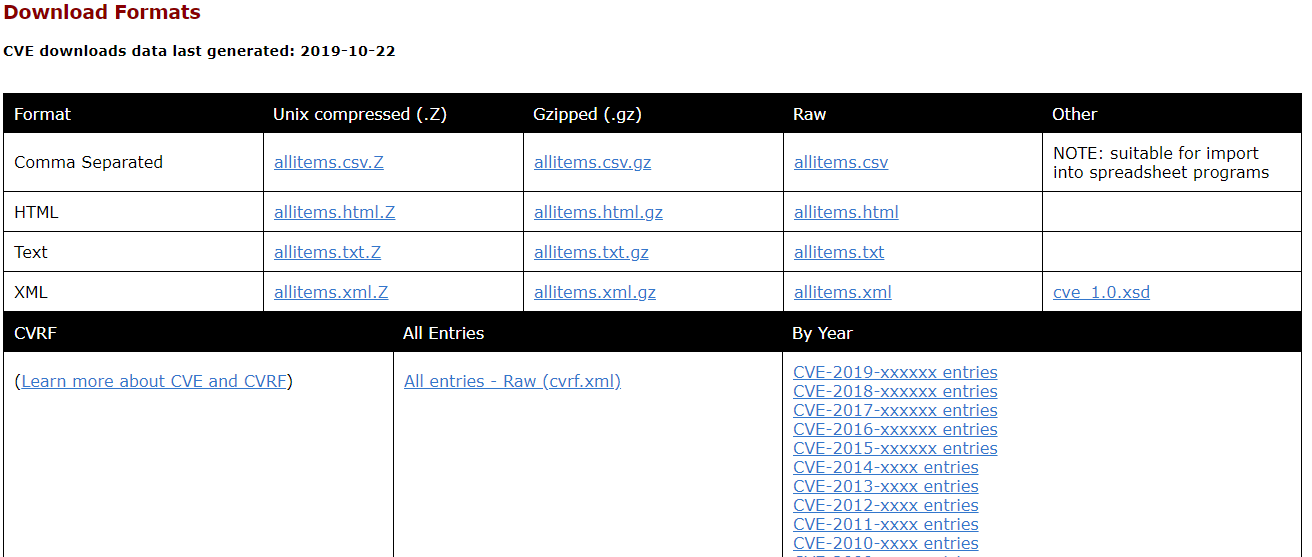
\includegraphics[width=1\textwidth]{imagens/cve_exemplo1.png}
\caption{Lista de opções de donwload de arquivos contendo vulnerabilidades}
\label{fig:cve1}
\end{figure}

Esses arquivos para download contém as vulnerabilidades do período selecionado. Caso selecionado o tipo, na primeira linha da tabela, é baixado todo um arquivo com aquela extensão selecionada e no formato desejado. Nesse arquivo será colocado todas as vulnerabilidades desde 1999. Quando baixado uma lista de vulnerabilidades de algum ano em específico, é carregado uma página web em xml com os dados daquele ano. A imagem \ref{fig:cve1_detalhes} mostra a configuração de um arquivo xml de exemplo.

\begin{figure}[H]
\centering
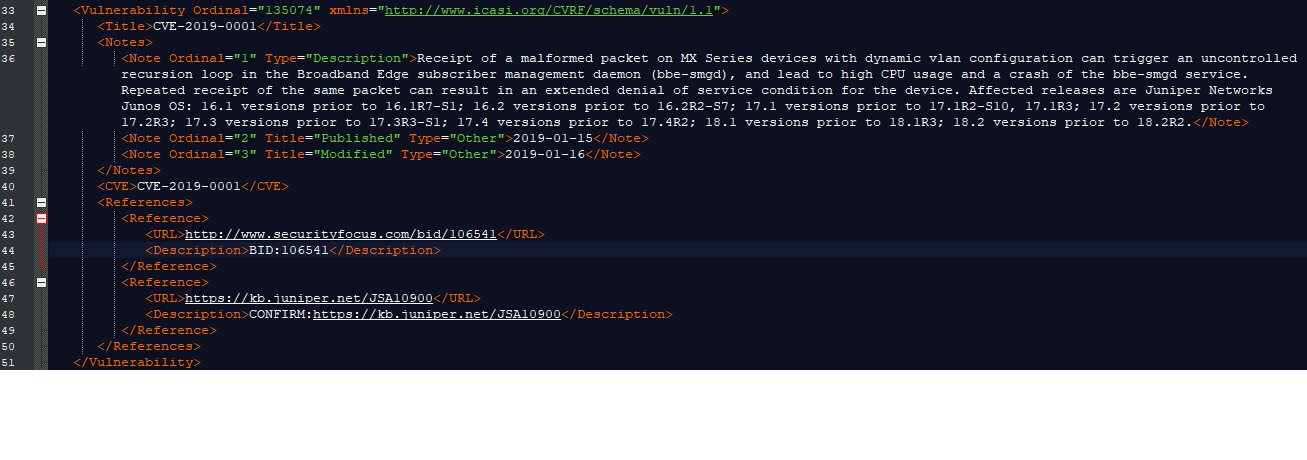
\includegraphics[width=1\textwidth]{imagens/cve1_detalhes.png}
\caption{Arquivo xml exemplificando uma vulnerabilidade de janeiro de 2019}
\label{fig:cve1_detalhes}
\end{figure}

Desse modo, o arquivo xml a ser baixado com as vulnerabilidades possibilita uma busca por códigos e até mesmo textos nas ocorrências, o que será utilizado no trabalho a fim de buscar os resultados com as postagens no twitter.

O site da NVD, entretanto, tem a possibilidade de listagem das vulnerabilidades através da seleção de um mês de algum ano, como apresentado na figura \ref{fig:nvd1}, filtrando o mês de setembro de 2019. Assim, é possível ter um filtro melhor caso esteja procurando apenas informações para uma leitura em específico.

\begin{figure}[H]
\centering
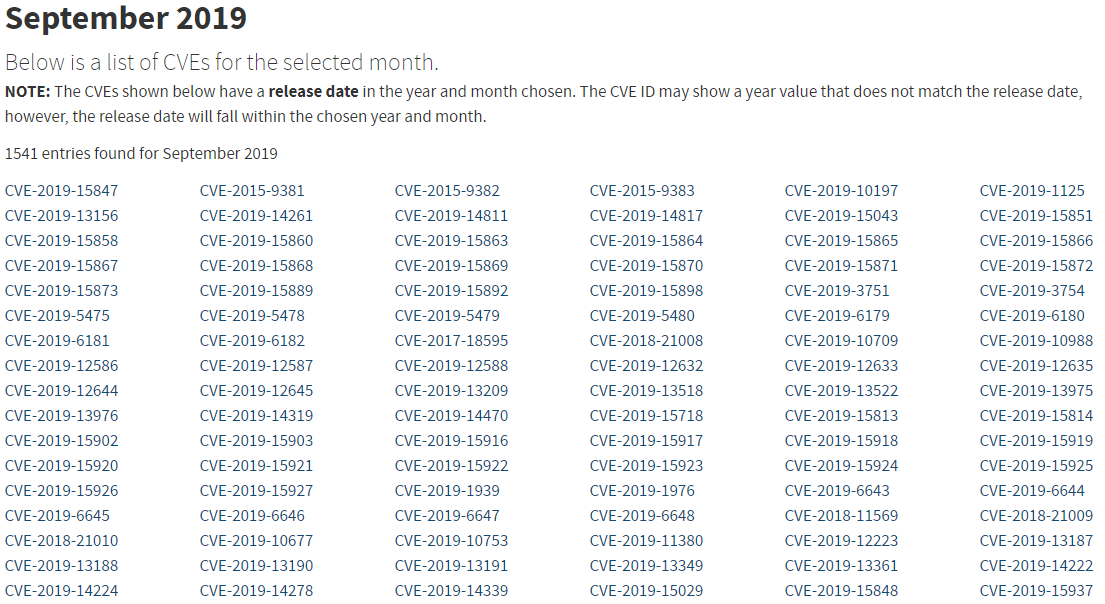
\includegraphics[width=1\textwidth]{imagens/nvd_exemplo1.png}
\caption{Vulnerabilidades reportadas pelo NVD em setembro de 2019}
\label{fig:nvd1}
\end{figure}

A Figura \ref{fig:nvd1} mostra parte das 1541 vulnerabilidades divulgadas para o mês de setembro de 2019. Quando selecionado algum CVE uma página é apresentando mostrando os detalhes daquela vulnerabilidade. Como um exemplo, o CVE-2019-15847 é apresentado na Figura \ref{fig:nvd3}.

\begin{figure}[H]
\centering
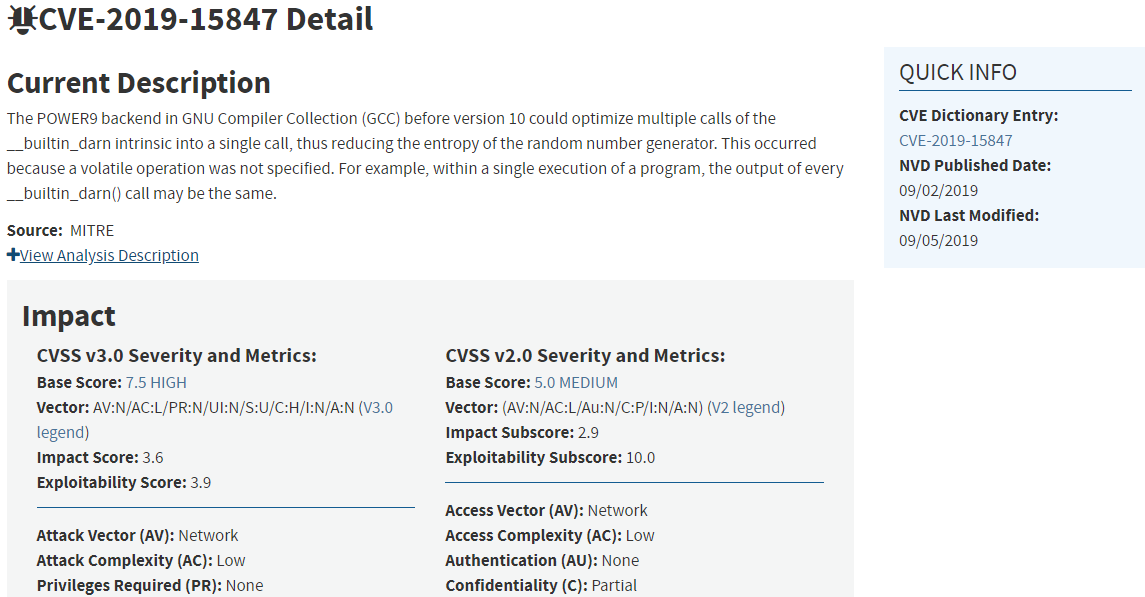
\includegraphics[width=1\textwidth]{imagens/nvd_exemplo3.png}
\caption{Vulnerabilidade CVE-2011-4042}
\label{fig:nvd3}
\end{figure}

A Figura \ref{fig:nvd3} apresenta os detalhes da vulnerabilidade CVE-2019-15847. Descrição \textit{(Description na Figura)}, a tabela de impacto \textit{(Impact na Figura)} e a data de publicação da vulnerabilidade \textit{(NVD Published Date na Figura)}, são alguns dos campos que são informados. Esses dados são oriundos do site da CVE e os mesmos arquivos xml que são possíveis de serem baixados são a base utilizada para a apresentação da informação. Logo, o site tem o proósito de apresentar a informação de uma forma mais legível e atraente para o usuário. 

O trabalho em questão utiliza esses dados do CVE como uma base de comparação de assuntos que estão postados no twitter. Dá-se então a estima para a listagem xml que possibilita uma mineração de dados em cima dos resultados obtidos do twitter.

% -------------------------------%
% --- Trabalhos Relacionados --- %
\section{Trabalhos Relacionados}

Esta seção tem o objetivo de descrever alguns trabalhos que têm relação ao tema principal desse projeto: discussão sobre vulnerabilidades em redes sociais. Os trabalhos \citeonline{Sabottke2015}, \citeonline{Correia2016}, \citeonline{ALVESBATISTA2007} e \citeonline{Kroth2018} serão apresentados posteriormente com o objetivo de descreve-los e vincula-los ao tema central desse trabalho. 

O número de vulnerabilidades tem crescido a cada ano, assim como é apresentado na figura \ref{fig:nvd1}, onde apenas no mês de setembro de 2019 é apresentado muitas novas incidências de bugs e backdoors. Esse crescimento é exponencial. Um outro exemplo que prova isso é que em 2014 foi o marco da primeira aparição de um CVE de 5 dígitos, pois o banco de dados do CVE [46], que atribui identificadores exclusivos às vulnerabilidades, adotou um novo formato que não limita mais o número de IDs do CVE a 10.000 por ano \cite{Sabottke2015}, assim é possível notar a quantidade crescente das vulnerabilidades, pois a nova métrica é incremental.

Um dos problemas é que esse crescimento de novas vulnerabilidades é muito maior que a capacidade de correções pela parte dos criadores \cite{ALVESBATISTA2007}. Nesse aspécto, tem-se a classificação qualitativa das vulnerabilidades encontradas. Essa classificação tem por objetivo identificar quais são as vulnerabilidades com  um nível de prioridade maior \cite{Sabottke2015}.

Com a ascensão do número de vulnerabilidades é necessário que haja aumento também do número de pessoas a combate-las. Nesse processo, o primeiro passo é identifica-las. As redes sociais estão nesse contexto, pois apresentam um meio que possibilita discussão sobre o assunto em questão. O Twitter, foco desse trabalho, é a rede social onde o assunto tem crescido, principalmente devido ao aumento de número de usuários, como apresentado na figura \ref{fig:relacionado_um}. em virtude das informações dos usuários obidas nessa rede social é possível, de forma automática, listar quais são as principais vulnerabilidades discutidas no momento e o quão importante elas são de serem sanadas e exploradas \cite{Correia2016}.

\begin{figure}[H]
\centering
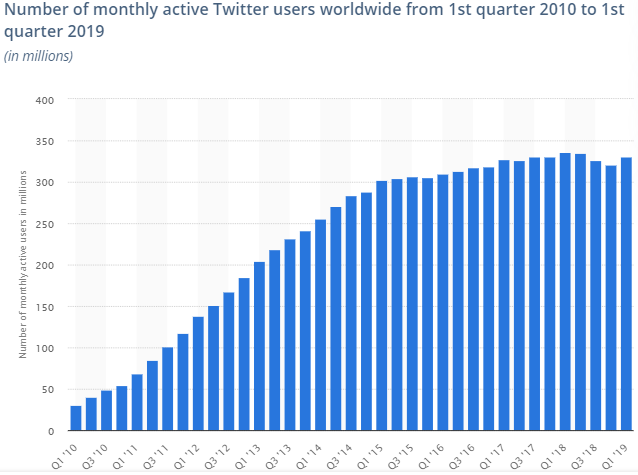
\includegraphics[width=1\textwidth]{imagens/relacionado_um.png}
\caption{Gráfico que apresenta o número de usuários na rede do Twitter entre os anos de 2010 e 2019 \cite{Statista2019}}
\label{fig:relacionado_um}
\end{figure}

\citeonline{Sabottke2015} é um trabalho que apresenta uma proposta de identificar, através de buscas no twitter, vulnerabilidades discutidas nessa rede social. Tem o objetivo de explorar qualitativa e quantitativamente os dados de vulnerabilidades disseminadas na rede \cite{Sabottke2015}. 

Muitas vulnerabilidades são encontradas e anunciadas diariamente. O capacidade de corrigir esses bugs é inversamente proporcional ao crescimento. \citeonline{Sabottke2015} então tenta propor uma forma de mensura das vulnerabilidades discutidas no Twitter, assim consegue levantar quais os problemas devem ser focadas primeiramente. Levanta também quais são os usuários que mantém essas discussões. Ademais, muitas das vulnerabilidades não têm grande impactos em sistemas, muitas vezes até sendo um falso-positivo, então o trabalho tem o objetivo de levantar apenas os bugs que realmente precisam ser corrigidos.

\citeonline{Sabottke2015} busca criar um sistema que filtre no tweets no Twitter através de alguma palavra chave e, a partir do resultado da busca, listar quais desses tweets falam sobre vulnerabilidades existentes e quais são exploráveis no mundo real. Para isso, o objetivo é criar um sistema que faça essa busca e essa sumarização qualitativa e quantitativa dos tweets, uma vez que essa tecnologia funcionará com a arquitetura apresentada na figura \ref{fig:Sabottke}.

\begin{figure}[H]
\centering
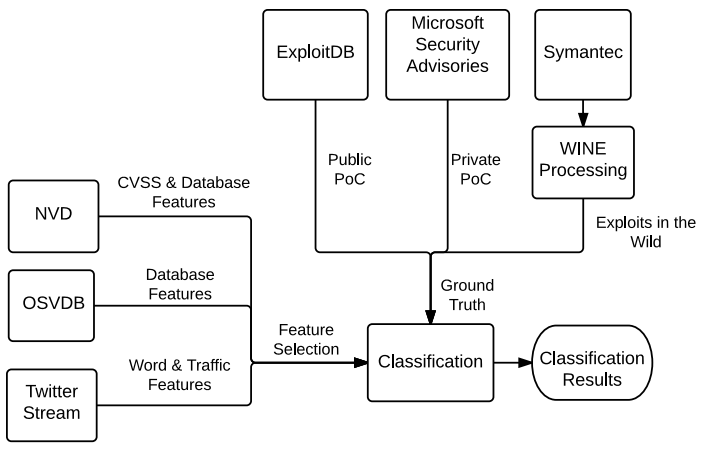
\includegraphics[width=1\textwidth]{imagens/Sabottke.png}
\caption{Arquitetura do sistema proposto pelo artigo \citeonline{Correia2016}}
\label{fig:Sabottke}
\end{figure}

Utilizando outras bases de segurança, o sistema se conecta à bases públicas como ExplitBD, Microsoft Security Advisories e Symantec, assim consegue filtrar as vulnerabilidades e buscar quais já foram exploradas. Essas bases de dados têm o objetivo de listar de forma organizada as vulnerabilidades com maior nível de atenção.

Assim, o sistema monta sua base de dados através do Twitter e faz a classificação, através das bases públicas de listagens de vulnerabilidades, de quais desses bugs devem ser tratados e fazendo o levantamento do quanto aparecem em publicações na rede social.

\citeonline{Correia2016} é um trabalho que utiliza de aprendizagem automática para conseguir identificar os tweets da rede social do Twitter que estão correlacionados à problemas de segurança de softwares e também relacionados à vulnerabilidades. Assim como \citeonline{Sabottke2015}, tem o objetivo de listar e filtrar de forma qualitativa e quantitativa as vulnerabilidades encontradas.

O autor tem como base o estudo de aprendizagem de máquina, uma vez que utiliza essa tecnologia com o objetivo de filtragem dos dados e, a partir dos resultados, melhorar a busca criando novos parâmetros para a pesquisa. O trabalho ainda lista uma série de restrições que a API utilizada para coleta dos dados tem, mas ainda sim apresenta seus resultados. A figura \ref{fig:Correia} apresenta a arquitetura utilizada para criação do sistema. Este é composto por duas fases, a representada a seguir é a fase de treino, onde é necessário o filtro humano para que o primeiro filtro seja feito. Essa necessidade se vê devido à natureza das técnicas de aprendizagem automáticas supervisionadas \cite{Correia2016}. Posterior a isso, o sistema consegue, através de aprendizagem, filtrar automaticamente os tweets de interesse. 

\begin{figure}[H]
\centering
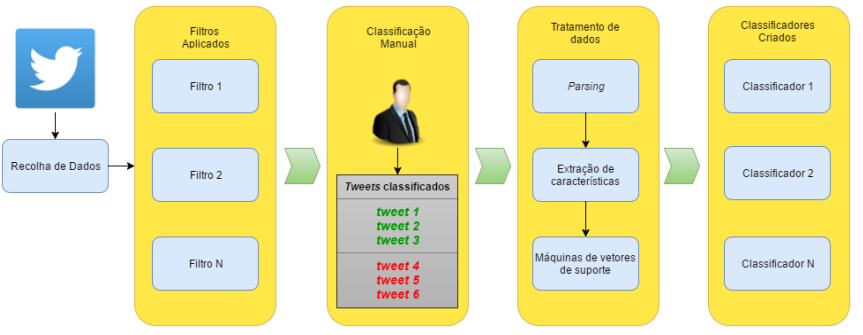
\includegraphics[width=1\textwidth]{imagens/Correia.png}
\caption{Arquitetura do sistema proposto pelo artigo \citeonline{Correia2016} representando a forma de treino do sistema}
\label{fig:Correia}
\end{figure}

Essa fase inicial tem o objetivo de, depois de recolidos os tweets, seja classificados por um analista quais são os dados relevantes em relação à ameaça de segurança à infraestrutura de TI. Após essa rotulação, o próprio sistema com os algoritmos de aprendizagem passa a conseguir um melhor resultado na obtenção de dados \cite{Correia2016}. Depois de treinado o sistema comporta de acordo com a arquitetura representada na figura \ref{fig:Correia2} no modo de operação.

\begin{figure}[H]
\centering
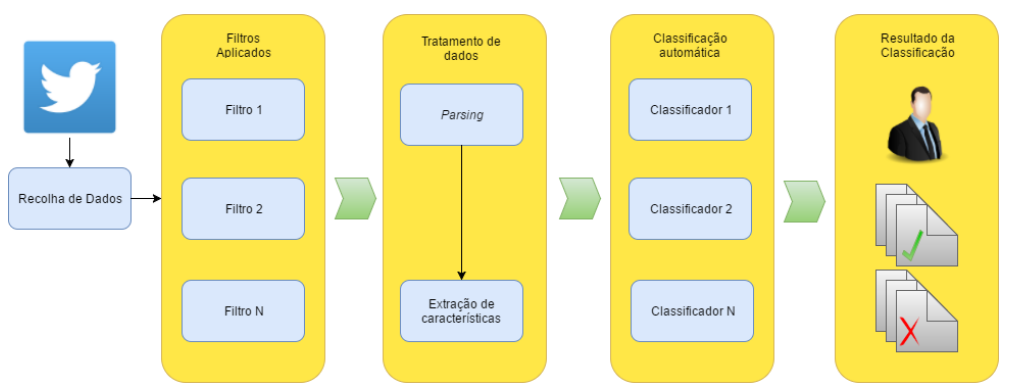
\includegraphics[width=1\textwidth]{imagens/Correia2.png}
\caption{Arquitetura do sistema proposto pelo artigo \citeonline{Correia2016} representando a forma de operação do sistema}
\label{fig:Correia2}
\end{figure}

Na fase de operação o sistema funciona de forma automática, após o treino ele consegue identificar melhor os filtros dos tweets, assim apresenta uma lista com os tweets selecionados que serão analisados por um analista posteriormente.

\citeonline{ALVESBATISTA2007} é um trabalho que estuda e apresenta dados sobre segurança em softwares e o quão difícil é de se abordar o tema colocando métricas de segurança, uma vez que nos dias atuais não é possível apresentar uma métrica quantitativa capaz de indicar o nível de segurança que o software em desenvolvimento terá \cite{ALVESBATISTA2007}. Esse trabalho tem o objetivo de comprovar essa teoria colocando a responsabilidade de segurança antes de se distribuir o software e assim sempre lançar um software fidedigno.

Com o objetivo de apresentar alguns métodos de avaliação quantitativa, apontando suas falhas, o trabalho propõe áreas de pesquisa para o estudo de métrica de seguranaça de software, para assim melhorar a avaliação. Desse modo, consegue-se a perspectiva do quão rentável é o investimento em segurança de software, a capacidade e competência de combater vulnerabilidades e como os riscos de segurança estão sendo gerenciados.

O trabalho define segurança como algo interpretativo e relativo. Quando se tem um cenário em que se coloca o nível de segurança X para um software, é relativo que a segurança do sistema tem que atende-lo no nível X. Como exemplo, um sistema de banco necessita de uma segurança alta em seu software, uma vez que um sistema de uma loja pequena de roupas de uma cidade de interior não precisa da mesma segurança. A métrica de segurança de um sistema, então, advem de sua necessidade de segurança e contexto de utilização.

\citeonline{Kroth2018} é um trabalho que busca identificar vulnerabilidades previamente definidas que estão presentes em serviços na internet, sendo esses públicos. Tem o objetivo de listar essas vulnerabilidades comuns que ataques utilizam para conseguirem acesso à informações de usuários.

O autor define que as vulnerabilidades disponíveis na rede advem de displicência por parte das organizações criadoras dos sistemas. Por parte delas o investimento em segurança não se baseia em resultado, sendo um custo sem retorno. Assim, os sistemas não têm um simples teste de invasão por uma equipe especializada, o que deixa ao público uma dúvida sobre o quão seguro o sistema é. O problema maior se encontra com o público que não conhece sobre segurança e disponibilizam seus dados em sistemas desse porte, que não tem o "selo de segurança".

O trabalho se baseia em delimitar a conexão da rede da Internet para uma rede LAN. Assim, o objetivo é encontrar vulnerabilidades previamente definidas na comunicação entre internet e LAN. Assim, o objetivo é identificar vulnerabilidade já conhecidas em sistemas em geral, contabilizando, assim, o número de sistemas que não se atualizaram, ou mesmo foram feitos, sob as medidas de segurança já definidas \cite{Kroth2018}.

Os trabahos citados têm focos diferentes nas perspectivas de segurança e objetivos diferentes. O trabalho \citeonline{Sabottke2015} e o \citeonline{Correia2016} são os que mais se aproximam com o presente trabalho, uma vez que faz também uma busca numa rede social em cima de palavras chaves e as explora para definição de vulnerabilidades em sistemas. Mas o trabalho \citeonline{ALVESBATISTA2007} se relaciona com o projeto sendo uma porta de caminho sobre o estudo de segurança do software, tendo sua base na métrica do quão um software pode ser mensurado como seguro, fazendo uma busca sobre o que seria seguro na definição de segurança de sistemas. O trabalho \citeonline{Kroth2018} também se destaco ao buscar vulnerabilidades já conhecidas pela sociedade em sistemas públicos, sendo essas vulnerabilidades já discutidas em redes sociais também. 

Existe ainda trabalhos que têm como parte do projeto a análise de dados de tweets, sendo muitos correlacionados à psicologia e estudo humano. Esses trabalho têm relação a esse pelo fato de buscar alguns filtros no Twitter. Se o presente trabalho faz uma busca por palavras chaves que retornam vulnerabilidades em sistemas, esses outros trabalhos apenas mudam a busca para conseguirem seu objetivo.